% Options for packages loaded elsewhere
\PassOptionsToPackage{unicode}{hyperref}
\PassOptionsToPackage{hyphens}{url}
%
\documentclass[
]{article}
\usepackage{lmodern}
\usepackage{amssymb,amsmath}
\usepackage{ifxetex,ifluatex}
\ifnum 0\ifxetex 1\fi\ifluatex 1\fi=0 % if pdftex
  \usepackage[T1]{fontenc}
  \usepackage[utf8]{inputenc}
  \usepackage{textcomp} % provide euro and other symbols
\else % if luatex or xetex
  \usepackage{unicode-math}
  \defaultfontfeatures{Scale=MatchLowercase}
  \defaultfontfeatures[\rmfamily]{Ligatures=TeX,Scale=1}
\fi
% Use upquote if available, for straight quotes in verbatim environments
\IfFileExists{upquote.sty}{\usepackage{upquote}}{}
\IfFileExists{microtype.sty}{% use microtype if available
  \usepackage[]{microtype}
  \UseMicrotypeSet[protrusion]{basicmath} % disable protrusion for tt fonts
}{}
\makeatletter
\@ifundefined{KOMAClassName}{% if non-KOMA class
  \IfFileExists{parskip.sty}{%
    \usepackage{parskip}
  }{% else
    \setlength{\parindent}{0pt}
    \setlength{\parskip}{6pt plus 2pt minus 1pt}}
}{% if KOMA class
  \KOMAoptions{parskip=half}}
\makeatother
\usepackage{xcolor}
\IfFileExists{xurl.sty}{\usepackage{xurl}}{} % add URL line breaks if available
\IfFileExists{bookmark.sty}{\usepackage{bookmark}}{\usepackage{hyperref}}
\hypersetup{
  pdftitle={Grammar of graphic for data visualisation},
  hidelinks,
  pdfcreator={LaTeX via pandoc}}
\urlstyle{same} % disable monospaced font for URLs
\usepackage[margin=1in]{geometry}
\usepackage{color}
\usepackage{fancyvrb}
\newcommand{\VerbBar}{|}
\newcommand{\VERB}{\Verb[commandchars=\\\{\}]}
\DefineVerbatimEnvironment{Highlighting}{Verbatim}{commandchars=\\\{\}}
% Add ',fontsize=\small' for more characters per line
\usepackage{framed}
\definecolor{shadecolor}{RGB}{248,248,248}
\newenvironment{Shaded}{\begin{snugshade}}{\end{snugshade}}
\newcommand{\AlertTok}[1]{\textcolor[rgb]{0.94,0.16,0.16}{#1}}
\newcommand{\AnnotationTok}[1]{\textcolor[rgb]{0.56,0.35,0.01}{\textbf{\textit{#1}}}}
\newcommand{\AttributeTok}[1]{\textcolor[rgb]{0.77,0.63,0.00}{#1}}
\newcommand{\BaseNTok}[1]{\textcolor[rgb]{0.00,0.00,0.81}{#1}}
\newcommand{\BuiltInTok}[1]{#1}
\newcommand{\CharTok}[1]{\textcolor[rgb]{0.31,0.60,0.02}{#1}}
\newcommand{\CommentTok}[1]{\textcolor[rgb]{0.56,0.35,0.01}{\textit{#1}}}
\newcommand{\CommentVarTok}[1]{\textcolor[rgb]{0.56,0.35,0.01}{\textbf{\textit{#1}}}}
\newcommand{\ConstantTok}[1]{\textcolor[rgb]{0.00,0.00,0.00}{#1}}
\newcommand{\ControlFlowTok}[1]{\textcolor[rgb]{0.13,0.29,0.53}{\textbf{#1}}}
\newcommand{\DataTypeTok}[1]{\textcolor[rgb]{0.13,0.29,0.53}{#1}}
\newcommand{\DecValTok}[1]{\textcolor[rgb]{0.00,0.00,0.81}{#1}}
\newcommand{\DocumentationTok}[1]{\textcolor[rgb]{0.56,0.35,0.01}{\textbf{\textit{#1}}}}
\newcommand{\ErrorTok}[1]{\textcolor[rgb]{0.64,0.00,0.00}{\textbf{#1}}}
\newcommand{\ExtensionTok}[1]{#1}
\newcommand{\FloatTok}[1]{\textcolor[rgb]{0.00,0.00,0.81}{#1}}
\newcommand{\FunctionTok}[1]{\textcolor[rgb]{0.00,0.00,0.00}{#1}}
\newcommand{\ImportTok}[1]{#1}
\newcommand{\InformationTok}[1]{\textcolor[rgb]{0.56,0.35,0.01}{\textbf{\textit{#1}}}}
\newcommand{\KeywordTok}[1]{\textcolor[rgb]{0.13,0.29,0.53}{\textbf{#1}}}
\newcommand{\NormalTok}[1]{#1}
\newcommand{\OperatorTok}[1]{\textcolor[rgb]{0.81,0.36,0.00}{\textbf{#1}}}
\newcommand{\OtherTok}[1]{\textcolor[rgb]{0.56,0.35,0.01}{#1}}
\newcommand{\PreprocessorTok}[1]{\textcolor[rgb]{0.56,0.35,0.01}{\textit{#1}}}
\newcommand{\RegionMarkerTok}[1]{#1}
\newcommand{\SpecialCharTok}[1]{\textcolor[rgb]{0.00,0.00,0.00}{#1}}
\newcommand{\SpecialStringTok}[1]{\textcolor[rgb]{0.31,0.60,0.02}{#1}}
\newcommand{\StringTok}[1]{\textcolor[rgb]{0.31,0.60,0.02}{#1}}
\newcommand{\VariableTok}[1]{\textcolor[rgb]{0.00,0.00,0.00}{#1}}
\newcommand{\VerbatimStringTok}[1]{\textcolor[rgb]{0.31,0.60,0.02}{#1}}
\newcommand{\WarningTok}[1]{\textcolor[rgb]{0.56,0.35,0.01}{\textbf{\textit{#1}}}}
\usepackage{graphicx,grffile}
\makeatletter
\def\maxwidth{\ifdim\Gin@nat@width>\linewidth\linewidth\else\Gin@nat@width\fi}
\def\maxheight{\ifdim\Gin@nat@height>\textheight\textheight\else\Gin@nat@height\fi}
\makeatother
% Scale images if necessary, so that they will not overflow the page
% margins by default, and it is still possible to overwrite the defaults
% using explicit options in \includegraphics[width, height, ...]{}
\setkeys{Gin}{width=\maxwidth,height=\maxheight,keepaspectratio}
% Set default figure placement to htbp
\makeatletter
\def\fps@figure{htbp}
\makeatother
\setlength{\emergencystretch}{3em} % prevent overfull lines
\providecommand{\tightlist}{%
  \setlength{\itemsep}{0pt}\setlength{\parskip}{0pt}}
\setcounter{secnumdepth}{-\maxdimen} % remove section numbering

\title{Grammar of graphic for data visualisation}
\author{}
\date{\vspace{-2.5em}}

\begin{document}
\maketitle

\begin{quote}
Dalam modul ini Anda akan menggunakan konsep Grammar of Graphics untuk
membuat visualisasi data.
\end{quote}

R merupakan bahasa pemrograman yang terkenal akan kemampuannya dalam
menghasilkan grafik atau visualisasi data dengan baik. Penting diketahui
bahwa R memiliki berbagai sistem dan paket untuk pembuatan grafik,
contohnya \texttt{base}, \texttt{lattice}, \texttt{ggplot}, dan
lain-lain. Namun dalam modul ini Akita akan fokus menggunakan sistem
\texttt{ggplot} untuk membuat visualisasi data.

Sistem pembuatan grafik dengan \texttt{ggplot} dapat dilakukan dengan
menggunakan paket \texttt{ggplot2} yang merupakan implementasi dari
konsep \emph{Grammar of graphic} untuk bahasa pemrograman R. Dengan
memahami konsep dari \emph{grammar of graphic}, kita dapat membuat
berbagai jenis plot dengan ringkas dan mudah. Sekarang aktifkanlah paket
\texttt{ggplot2} tersebut terlebih dahulu!

\begin{Shaded}
\begin{Highlighting}[]
\KeywordTok{library}\NormalTok{(ggplot2)}
\end{Highlighting}
\end{Shaded}

Dalam contoh ini Anda akan membuat grafik dari dataset \texttt{diamonds}
yang tersedia dalam paket \texttt{ggplot2}. Anda dapat melihat isi serta
dokumentasi dari dataset tersebut dengan menjalankan \texttt{diamonds}
dan \texttt{?diamonds}. Berisi informasi apakah data \texttt{diamonds}?
Silakan lakukan inspeksi pada struktur data tersebut!

\begin{Shaded}
\begin{Highlighting}[]
\NormalTok{diamonds}
\CommentTok{#> # A tibble: 53,940 x 10}
\CommentTok{#>    carat cut       color clarity depth table price     x     y     z}
\CommentTok{#>    <dbl> <ord>     <ord> <ord>   <dbl> <dbl> <int> <dbl> <dbl> <dbl>}
\CommentTok{#>  1 0.23  Ideal     E     SI2      61.5    55   326  3.95  3.98  2.43}
\CommentTok{#>  2 0.21  Premium   E     SI1      59.8    61   326  3.89  3.84  2.31}
\CommentTok{#>  3 0.23  Good      E     VS1      56.9    65   327  4.05  4.07  2.31}
\CommentTok{#>  4 0.290 Premium   I     VS2      62.4    58   334  4.2   4.23  2.63}
\CommentTok{#>  5 0.31  Good      J     SI2      63.3    58   335  4.34  4.35  2.75}
\CommentTok{#>  6 0.24  Very Good J     VVS2     62.8    57   336  3.94  3.96  2.48}
\CommentTok{#>  7 0.24  Very Good I     VVS1     62.3    57   336  3.95  3.98  2.47}
\CommentTok{#>  8 0.26  Very Good H     SI1      61.9    55   337  4.07  4.11  2.53}
\CommentTok{#>  9 0.22  Fair      E     VS2      65.1    61   337  3.87  3.78  2.49}
\CommentTok{#> 10 0.23  Very Good H     VS1      59.4    61   338  4     4.05  2.39}
\CommentTok{#> # ... with 53,930 more rows}
\NormalTok{?diamonds}
\CommentTok{#> starting httpd help server ... done}
\KeywordTok{str}\NormalTok{(diamonds)}
\CommentTok{#> Classes 'tbl_df', 'tbl' and 'data.frame':    53940 obs. of  10 variables:}
\CommentTok{#>  $ carat  : num  0.23 0.21 0.23 0.29 0.31 0.24 0.24 0.26 0.22 0.23 ...}
\CommentTok{#>  $ cut    : Ord.factor w/ 5 levels "Fair"<"Good"<..: 5 4 2 4 2 3 3 3 1 3 ...}
\CommentTok{#>  $ color  : Ord.factor w/ 7 levels "D"<"E"<"F"<"G"<..: 2 2 2 6 7 7 6 5 2 5 ...}
\CommentTok{#>  $ clarity: Ord.factor w/ 8 levels "I1"<"SI2"<"SI1"<..: 2 3 5 4 2 6 7 3 4 5 ...}
\CommentTok{#>  $ depth  : num  61.5 59.8 56.9 62.4 63.3 62.8 62.3 61.9 65.1 59.4 ...}
\CommentTok{#>  $ table  : num  55 61 65 58 58 57 57 55 61 61 ...}
\CommentTok{#>  $ price  : int  326 326 327 334 335 336 336 337 337 338 ...}
\CommentTok{#>  $ x      : num  3.95 3.89 4.05 4.2 4.34 3.94 3.95 4.07 3.87 4 ...}
\CommentTok{#>  $ y      : num  3.98 3.84 4.07 4.23 4.35 3.96 3.98 4.11 3.78 4.05 ...}
\CommentTok{#>  $ z      : num  2.43 2.31 2.31 2.63 2.75 2.48 2.47 2.53 2.49 2.39 ...}
\end{Highlighting}
\end{Shaded}

Kita dapat menggunakan fungsi \texttt{qplot()} untuk membuat grafik
menggunakan \texttt{ggplot2}. Bacalah terlebih dahulu dokumentasi fungsi
\texttt{qplot()} dan kemudian lengkapilah \emph{chunk} berikut untuk
membuat grafik hubungan antara berat (sumbu x), harga (sumbu y) dan
kejernihan intan (variasi warna) dari dataset diamonds!

\begin{Shaded}
\begin{Highlighting}[]
\KeywordTok{qplot}\NormalTok{(}\DataTypeTok{x =}\NormalTok{ carat, }\DataTypeTok{y =}\NormalTok{ price, }\DataTypeTok{colour =}\NormalTok{  clarity, }\DataTypeTok{data =}\NormalTok{ diamonds)}
\end{Highlighting}
\end{Shaded}

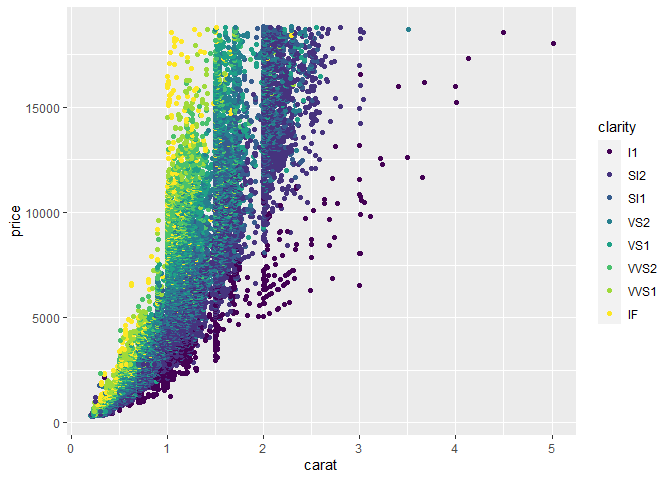
\includegraphics{modul8_files/figure-latex/unnamed-chunk-3-1.pdf}

Pembuatan grafik dengan menggunakan fungsi \texttt{qplot()} memang
relatif mudah, namun fiturnya terbatas dan kurang fleksibel. Oleh karena
itu, kita akan mempelajari dan menggunakan fungsi \texttt{ggplot()}
untuk membuat visualisasi data dengan lebih leluasa. Grafik diatas dapat
diolah kembali dengan menggunakan penulisan kode sebagai berikut::

\begin{Shaded}
\begin{Highlighting}[]
\KeywordTok{ggplot}\NormalTok{(}\DataTypeTok{data =}\NormalTok{ diamonds, }\DataTypeTok{mapping =} \KeywordTok{aes}\NormalTok{(}\DataTypeTok{x =}\NormalTok{ carat, }\DataTypeTok{y =}\NormalTok{ price, }\DataTypeTok{colour =}\NormalTok{ clarity)) }\OperatorTok{+}
\StringTok{  }\KeywordTok{geom_point}\NormalTok{()}
\end{Highlighting}
\end{Shaded}

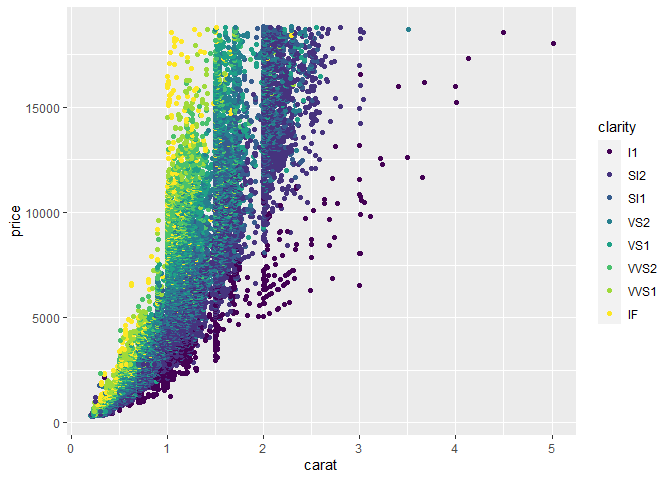
\includegraphics{modul8_files/figure-latex/unnamed-chunk-4-1.pdf}

Hal yang menarik dan membedakan antara pembuatan grafik menggunakan
\texttt{ggplot2} dan \texttt{base} adalah bahwa keluaran fungsi
\texttt{ggplot()} dapat disimpan sebagai obyek R. Apa manfaatnya?
Pertama adalah kita dapat dengan mudah menyimpan grafik seperti halnya
menjalankan \texttt{write.csv()} pada dataset. Kedua adalah kita dapat
dengan leluasa melakukan modifikasi pada grafik yang telah dibuat. Hal
ini akan dibahas dalam subbagian kedepan.

Baris kode dalam \emph{chunk} berikut menunjukan cara untuk menyimpan
grafik ke dalam obyek R bernama \texttt{plot\_diamonds} dan kemudian
menyimpannya dalam komputer dengan nama berkas ``diamonds.png''. Kita
akan menggunakan fungsi \texttt{ggsave()} yang juga berasal dari paket
\texttt{ggplot2}.

\begin{Shaded}
\begin{Highlighting}[]
\NormalTok{plot_diamonds <-}\StringTok{ }\KeywordTok{ggplot}\NormalTok{(}\DataTypeTok{data =}\NormalTok{ diamonds) }\OperatorTok{+}
\StringTok{  }\KeywordTok{geom_point}\NormalTok{(}\DataTypeTok{mapping =} \KeywordTok{aes}\NormalTok{(}\DataTypeTok{x =}\NormalTok{ carat, }\DataTypeTok{y =}\NormalTok{ price, }\DataTypeTok{colour =}\NormalTok{ clarity)) }\CommentTok{# Saat output disimpan ke dalam obyek R, grafik tidak otomatis dicetak pada layar}

\NormalTok{plot_diamonds }\CommentTok{# Untuk mencetak grafik, Anda harus menjalankan nama obyek R yang sebelumnya dibuat}
\end{Highlighting}
\end{Shaded}

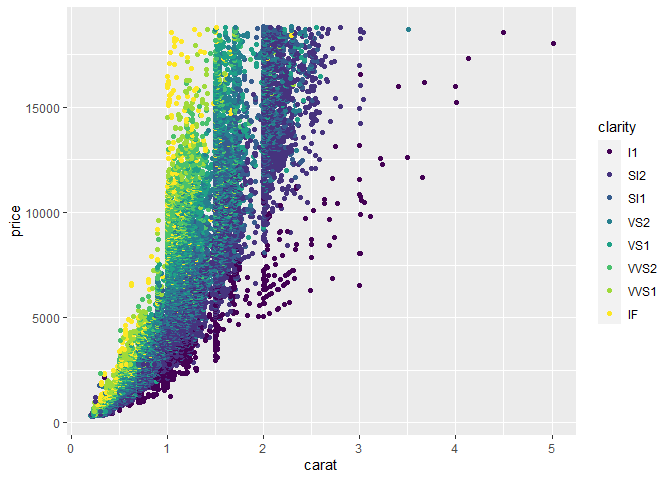
\includegraphics{modul8_files/figure-latex/unnamed-chunk-5-1.pdf}

\begin{Shaded}
\begin{Highlighting}[]

\KeywordTok{ggsave}\NormalTok{(}\DataTypeTok{filename =} \StringTok{"diamonds.jpg"}\NormalTok{, }\DataTypeTok{plot =}\NormalTok{ plot_diamonds)}
\CommentTok{#> Saving 6.5 x 4.5 in image}
\end{Highlighting}
\end{Shaded}

Meskipun penulisan kode R untuk membuat grafik menggunakan fungsi
\texttt{ggplot()} relatif lebih panjang, lebih banyak kostumisasi dan
pengaturan grafik yang dapat dilakukan dengan menggunakan fungsi
\texttt{ggplot()} dibandingkan fungsi \texttt{qplot()}. Dalam pelatihan
ini Anda akan diminta untuk membuat banyak grafik dengan menggunakan
struktur penulisan kode sebagai berikut:

\begin{verbatim}
ggplot(data = <DATA>) +
  <GEOM_FUNCTION>(mapping = aes(<MAPPINGS>))
\end{verbatim}

Dapat ditarik kesimpulan berdasarkan struktur penulisan kode R di atas
bahwa setidaknya terdapat tiga komponen utama untuk membuat grafik,
yaitu:

\begin{enumerate}
\def\labelenumi{\arabic{enumi}.}
\tightlist
\item
  \emph{Data}
\item
  \emph{Aesthetic mapping}
\item
  \emph{Geometric object}
\end{enumerate}

Pelajarilah dokumentasi fungsi \texttt{aes()} dan \texttt{geom\_point()}
(sebagai salah satu contoh \emph{geometric object}) melalui kode
berikut!

\begin{Shaded}
\begin{Highlighting}[]
\NormalTok{?aes}
\NormalTok{?geom_point}
\end{Highlighting}
\end{Shaded}

Selanjutnya kita akan bereksperimen membuat visualisasi data Ujian
Nasional tingkat SMP di Kota Bandung yang disediakan oleh
\href{http://data.bandung.go.id}{Open Data Kota Bandung}. Data tersebut
tersedia sebagai berkas ``un\_smp.csv'' dalam subdirektori ``data-raw''.
Silakan impor data tersebut sebagai obyek R bernama \texttt{un\_smp}
menggunakan fungsi \texttt{vroom()} dan \texttt{here()} dan cetaklah
pada layar! (Petunjuk: aktifkan terlebih dahulu paket-paket yang
relevan)

\begin{Shaded}
\begin{Highlighting}[]
\KeywordTok{library}\NormalTok{(vroom)}
\CommentTok{#> Warning: package 'vroom' was built under R version 3.6.3}
\KeywordTok{library}\NormalTok{(here)}
\CommentTok{#> Warning: package 'here' was built under R version 3.6.3}
\CommentTok{#> here() starts at C:/Users/HP/Documents}
\end{Highlighting}
\end{Shaded}

\begin{Shaded}
\begin{Highlighting}[]
\NormalTok{un_smp <-}\StringTok{ }\KeywordTok{vroom}\NormalTok{(}\KeywordTok{here}\NormalTok{(}\StringTok{"Kuliah/Semester 6/Praktikum Data Science/Praktikum 8"}\NormalTok{, }\StringTok{"un_smp.csv"}\NormalTok{))}
\CommentTok{#> Rows: 1,409}
\CommentTok{#> Columns: 8}
\CommentTok{#> Delimiter: ","}
\CommentTok{#> chr [2]: status, nama_sekolah}
\CommentTok{#> dbl [6]: tahun, jumlah_peserta, bahasa_indonesia, bahasa_inggris, matematika, ipa}
\CommentTok{#> }
\CommentTok{#> Use `spec()` to retrieve the guessed column specification}
\CommentTok{#> Pass a specification to the `col_types` argument to quiet this message}
\NormalTok{un_smp}
\CommentTok{#> # A tibble: 1,409 x 8}
\CommentTok{#>    tahun status nama_sekolah jumlah_peserta bahasa_indonesia bahasa_inggris}
\CommentTok{#>    <dbl> <chr>  <chr>                 <dbl>            <dbl>          <dbl>}
\CommentTok{#>  1  2015 Negeri SMP NEGERI ~            441             86.5           82.3}
\CommentTok{#>  2  2015 Negeri SMP NEGERI ~            284             86.4           88.7}
\CommentTok{#>  3  2015 Negeri SMP NEGERI ~            291             86.2           81.4}
\CommentTok{#>  4  2015 Negeri SMP NEGERI ~            385             84.5           77.8}
\CommentTok{#>  5  2015 Negeri SMP NEGERI ~            333             89.2           91.3}
\CommentTok{#>  6  2015 Negeri SMP NEGERI ~            341             77.2           64.3}
\CommentTok{#>  7  2015 Negeri SMP NEGERI ~            352             86.4           86.3}
\CommentTok{#>  8  2015 Negeri SMP NEGERI ~            317             84.3           80.4}
\CommentTok{#>  9  2015 Negeri SMP NEGERI ~            450             83.4           78.2}
\CommentTok{#> 10  2015 Negeri SMP NEGERI ~            353             78.4           70.3}
\CommentTok{#> # ... with 1,399 more rows, and 2 more variables: matematika <dbl>, ipa <dbl>}
\end{Highlighting}
\end{Shaded}

Pelajarilah struktur data \texttt{un\_smp} tersebut. Ada berapa
observasi dan variabel yang tersedia? Apa saja nama dari setiap kolom?
Data tahun berapa sajakah yang tersedia pada data tersebut?

\begin{Shaded}
\begin{Highlighting}[]
\KeywordTok{length}\NormalTok{(un_smp)}
\CommentTok{#> [1] 8}
\KeywordTok{names}\NormalTok{(un_smp)}
\CommentTok{#> [1] "tahun"            "status"           "nama_sekolah"     "jumlah_peserta"  }
\CommentTok{#> [5] "bahasa_indonesia" "bahasa_inggris"   "matematika"       "ipa"}
\NormalTok{un_smp}\OperatorTok{$}\NormalTok{tahun}
\CommentTok{#>    [1] 2015 2015 2015 2015 2015 2015 2015 2015 2015 2015 2015 2015 2015 2015}
\CommentTok{#>   [15] 2015 2015 2015 2015 2015 2015 2015 2015 2015 2015 2015 2015 2015 2015}
\CommentTok{#>   [29] 2015 2015 2015 2015 2015 2015 2015 2015 2015 2015 2015 2015 2015 2015}
\CommentTok{#>   [43] 2015 2015 2015 2015 2015 2015 2015 2015 2015 2015 2015 2015 2015 2015}
\CommentTok{#>   [57] 2015 2015 2015 2015 2015 2015 2015 2015 2015 2015 2015 2015 2015 2015}
\CommentTok{#>   [71] 2015 2015 2015 2015 2015 2015 2015 2015 2015 2015 2015 2015 2015 2015}
\CommentTok{#>   [85] 2015 2015 2015 2015 2015 2015 2015 2015 2015 2015 2015 2015 2015 2015}
\CommentTok{#>   [99] 2015 2015 2015 2015 2015 2015 2015 2015 2015 2015 2015 2015 2015 2015}
\CommentTok{#>  [113] 2015 2015 2015 2015 2015 2015 2015 2015 2015 2015 2015 2015 2015 2015}
\CommentTok{#>  [127] 2015 2015 2015 2015 2015 2015 2015 2015 2015 2015 2015 2015 2015 2015}
\CommentTok{#>  [141] 2015 2015 2015 2015 2015 2015 2015 2015 2015 2015 2015 2015 2015 2015}
\CommentTok{#>  [155] 2015 2015 2015 2015 2015 2015 2015 2015 2015 2015 2015 2015 2015 2015}
\CommentTok{#>  [169] 2015 2015 2015 2015 2015 2015 2015 2015 2015 2015 2015 2015 2015 2015}
\CommentTok{#>  [183] 2015 2015 2015 2015 2015 2015 2015 2015 2015 2015 2015 2015 2015 2015}
\CommentTok{#>  [197] 2015 2015 2015 2015 2015 2015 2015 2015 2015 2015 2015 2015 2015 2015}
\CommentTok{#>  [211] 2015 2015 2015 2015 2015 2015 2015 2015 2015 2015 2015 2015 2015 2015}
\CommentTok{#>  [225] 2015 2015 2015 2015 2015 2015 2015 2015 2015 2015 2015 2015 2015 2015}
\CommentTok{#>  [239] 2015 2015 2015 2015 2015 2015 2015 2015 2015 2015 2015 2015 2015 2015}
\CommentTok{#>  [253] 2015 2015 2015 2015 2015 2015 2015 2015 2015 2015 2015 2015 2015 2015}
\CommentTok{#>  [267] 2015 2015 2015 2015 2016 2016 2016 2016 2016 2016 2016 2016 2016 2016}
\CommentTok{#>  [281] 2016 2016 2016 2016 2016 2016 2016 2016 2016 2016 2016 2016 2016 2016}
\CommentTok{#>  [295] 2016 2016 2016 2016 2016 2016 2016 2016 2016 2016 2016 2016 2016 2016}
\CommentTok{#>  [309] 2016 2016 2016 2016 2016 2016 2016 2016 2016 2016 2016 2016 2016 2016}
\CommentTok{#>  [323] 2016 2016 2016 2016 2016 2016 2016 2016 2016 2016 2016 2016 2016 2016}
\CommentTok{#>  [337] 2016 2016 2016 2016 2016 2016 2016 2016 2016 2016 2016 2016 2016 2016}
\CommentTok{#>  [351] 2016 2016 2016 2016 2016 2016 2016 2016 2016 2016 2016 2016 2016 2016}
\CommentTok{#>  [365] 2016 2016 2016 2016 2016 2016 2016 2016 2016 2016 2016 2016 2016 2016}
\CommentTok{#>  [379] 2016 2016 2016 2016 2016 2016 2016 2016 2016 2016 2016 2016 2016 2016}
\CommentTok{#>  [393] 2016 2016 2016 2016 2016 2016 2016 2016 2016 2016 2016 2016 2016 2016}
\CommentTok{#>  [407] 2016 2016 2016 2016 2016 2016 2016 2016 2016 2016 2016 2016 2016 2016}
\CommentTok{#>  [421] 2016 2016 2016 2016 2016 2016 2016 2016 2016 2016 2016 2016 2016 2016}
\CommentTok{#>  [435] 2016 2016 2016 2016 2016 2016 2016 2016 2016 2016 2016 2016 2016 2016}
\CommentTok{#>  [449] 2016 2016 2016 2016 2016 2016 2016 2016 2016 2016 2016 2016 2016 2016}
\CommentTok{#>  [463] 2016 2016 2016 2016 2016 2016 2016 2016 2016 2016 2016 2016 2016 2016}
\CommentTok{#>  [477] 2016 2016 2016 2016 2016 2016 2016 2016 2016 2016 2016 2016 2016 2016}
\CommentTok{#>  [491] 2016 2016 2016 2016 2016 2016 2016 2016 2016 2016 2016 2016 2016 2016}
\CommentTok{#>  [505] 2016 2016 2016 2016 2016 2016 2016 2016 2016 2016 2016 2016 2016 2016}
\CommentTok{#>  [519] 2016 2016 2016 2016 2016 2016 2016 2016 2016 2016 2016 2016 2016 2016}
\CommentTok{#>  [533] 2016 2016 2016 2016 2016 2016 2016 2016 2016 2016 2016 2016 2016 2016}
\CommentTok{#>  [547] 2016 2016 2017 2017 2017 2017 2017 2017 2017 2017 2017 2017 2017 2017}
\CommentTok{#>  [561] 2017 2017 2017 2017 2017 2017 2017 2017 2017 2017 2017 2017 2017 2017}
\CommentTok{#>  [575] 2017 2017 2017 2017 2017 2017 2017 2017 2017 2017 2017 2017 2017 2017}
\CommentTok{#>  [589] 2017 2017 2017 2017 2017 2017 2017 2017 2017 2017 2017 2017 2017 2017}
\CommentTok{#>  [603] 2017 2017 2017 2017 2017 2017 2017 2017 2017 2017 2017 2017 2017 2017}
\CommentTok{#>  [617] 2017 2017 2017 2017 2017 2017 2017 2017 2017 2017 2017 2017 2017 2017}
\CommentTok{#>  [631] 2017 2017 2017 2017 2017 2017 2017 2017 2017 2017 2017 2017 2017 2017}
\CommentTok{#>  [645] 2017 2017 2017 2017 2017 2017 2017 2017 2017 2017 2017 2017 2017 2017}
\CommentTok{#>  [659] 2017 2017 2017 2017 2017 2017 2017 2017 2017 2017 2017 2017 2017 2017}
\CommentTok{#>  [673] 2017 2017 2017 2017 2017 2017 2017 2017 2017 2017 2017 2017 2017 2017}
\CommentTok{#>  [687] 2017 2017 2017 2017 2017 2017 2017 2017 2017 2017 2017 2017 2017 2017}
\CommentTok{#>  [701] 2017 2017 2017 2017 2017 2017 2017 2017 2017 2017 2017 2017 2017 2017}
\CommentTok{#>  [715] 2017 2017 2017 2017 2017 2017 2017 2017 2017 2017 2017 2017 2017 2017}
\CommentTok{#>  [729] 2017 2017 2017 2017 2017 2017 2017 2017 2017 2017 2017 2017 2017 2017}
\CommentTok{#>  [743] 2017 2017 2017 2017 2017 2017 2017 2017 2017 2017 2017 2017 2017 2017}
\CommentTok{#>  [757] 2017 2017 2017 2017 2017 2017 2017 2017 2017 2017 2017 2017 2017 2017}
\CommentTok{#>  [771] 2017 2017 2017 2017 2017 2017 2017 2017 2017 2017 2017 2017 2017 2017}
\CommentTok{#>  [785] 2017 2017 2017 2017 2017 2017 2017 2017 2017 2017 2017 2017 2017 2017}
\CommentTok{#>  [799] 2017 2017 2017 2017 2017 2017 2017 2017 2017 2017 2017 2017 2017 2017}
\CommentTok{#>  [813] 2017 2017 2017 2017 2017 2017 2017 2017 2017 2017 2017 2017 2017 2017}
\CommentTok{#>  [827] 2017 2017 2017 2017 2017 2018 2018 2018 2018 2018 2018 2018 2018 2018}
\CommentTok{#>  [841] 2018 2018 2018 2018 2018 2018 2018 2018 2018 2018 2018 2018 2018 2018}
\CommentTok{#>  [855] 2018 2018 2018 2018 2018 2018 2018 2018 2018 2018 2018 2018 2018 2018}
\CommentTok{#>  [869] 2018 2018 2018 2018 2018 2018 2018 2018 2018 2018 2018 2018 2018 2018}
\CommentTok{#>  [883] 2018 2018 2018 2018 2018 2018 2018 2018 2018 2018 2018 2018 2018 2018}
\CommentTok{#>  [897] 2018 2018 2018 2018 2018 2018 2018 2018 2018 2018 2018 2018 2018 2018}
\CommentTok{#>  [911] 2018 2018 2018 2018 2018 2018 2018 2018 2018 2018 2018 2018 2018 2018}
\CommentTok{#>  [925] 2018 2018 2018 2018 2018 2018 2018 2018 2018 2018 2018 2018 2018 2018}
\CommentTok{#>  [939] 2018 2018 2018 2018 2018 2018 2018 2018 2018 2018 2018 2018 2018 2018}
\CommentTok{#>  [953] 2018 2018 2018 2018 2018 2018 2018 2018 2018 2018 2018 2018 2018 2018}
\CommentTok{#>  [967] 2018 2018 2018 2018 2018 2018 2018 2018 2018 2018 2018 2018 2018 2018}
\CommentTok{#>  [981] 2018 2018 2018 2018 2018 2018 2018 2018 2018 2018 2018 2018 2018 2018}
\CommentTok{#>  [995] 2018 2018 2018 2018 2018 2018 2018 2018 2018 2018 2018 2018 2018 2018}
\CommentTok{#> [1009] 2018 2018 2018 2018 2018 2018 2018 2018 2018 2018 2018 2018 2018 2018}
\CommentTok{#> [1023] 2018 2018 2018 2018 2018 2018 2018 2018 2018 2018 2018 2018 2018 2018}
\CommentTok{#> [1037] 2018 2018 2018 2018 2018 2018 2018 2018 2018 2018 2018 2018 2018 2018}
\CommentTok{#> [1051] 2018 2018 2018 2018 2018 2018 2018 2018 2018 2018 2018 2018 2018 2018}
\CommentTok{#> [1065] 2018 2018 2018 2018 2018 2018 2018 2018 2018 2018 2018 2018 2018 2018}
\CommentTok{#> [1079] 2018 2018 2018 2018 2018 2018 2018 2018 2018 2018 2018 2018 2018 2018}
\CommentTok{#> [1093] 2018 2018 2018 2018 2018 2018 2018 2018 2018 2018 2018 2018 2018 2018}
\CommentTok{#> [1107] 2018 2018 2018 2018 2018 2018 2018 2018 2018 2018 2018 2018 2019 2019}
\CommentTok{#> [1121] 2019 2019 2019 2019 2019 2019 2019 2019 2019 2019 2019 2019 2019 2019}
\CommentTok{#> [1135] 2019 2019 2019 2019 2019 2019 2019 2019 2019 2019 2019 2019 2019 2019}
\CommentTok{#> [1149] 2019 2019 2019 2019 2019 2019 2019 2019 2019 2019 2019 2019 2019 2019}
\CommentTok{#> [1163] 2019 2019 2019 2019 2019 2019 2019 2019 2019 2019 2019 2019 2019 2019}
\CommentTok{#> [1177] 2019 2019 2019 2019 2019 2019 2019 2019 2019 2019 2019 2019 2019 2019}
\CommentTok{#> [1191] 2019 2019 2019 2019 2019 2019 2019 2019 2019 2019 2019 2019 2019 2019}
\CommentTok{#> [1205] 2019 2019 2019 2019 2019 2019 2019 2019 2019 2019 2019 2019 2019 2019}
\CommentTok{#> [1219] 2019 2019 2019 2019 2019 2019 2019 2019 2019 2019 2019 2019 2019 2019}
\CommentTok{#> [1233] 2019 2019 2019 2019 2019 2019 2019 2019 2019 2019 2019 2019 2019 2019}
\CommentTok{#> [1247] 2019 2019 2019 2019 2019 2019 2019 2019 2019 2019 2019 2019 2019 2019}
\CommentTok{#> [1261] 2019 2019 2019 2019 2019 2019 2019 2019 2019 2019 2019 2019 2019 2019}
\CommentTok{#> [1275] 2019 2019 2019 2019 2019 2019 2019 2019 2019 2019 2019 2019 2019 2019}
\CommentTok{#> [1289] 2019 2019 2019 2019 2019 2019 2019 2019 2019 2019 2019 2019 2019 2019}
\CommentTok{#> [1303] 2019 2019 2019 2019 2019 2019 2019 2019 2019 2019 2019 2019 2019 2019}
\CommentTok{#> [1317] 2019 2019 2019 2019 2019 2019 2019 2019 2019 2019 2019 2019 2019 2019}
\CommentTok{#> [1331] 2019 2019 2019 2019 2019 2019 2019 2019 2019 2019 2019 2019 2019 2019}
\CommentTok{#> [1345] 2019 2019 2019 2019 2019 2019 2019 2019 2019 2019 2019 2019 2019 2019}
\CommentTok{#> [1359] 2019 2019 2019 2019 2019 2019 2019 2019 2019 2019 2019 2019 2019 2019}
\CommentTok{#> [1373] 2019 2019 2019 2019 2019 2019 2019 2019 2019 2019 2019 2019 2019 2019}
\CommentTok{#> [1387] 2019 2019 2019 2019 2019 2019 2019 2019 2019 2019 2019 2019 2019 2019}
\CommentTok{#> [1401] 2019 2019 2019 2019 2019 2019 2019 2019 2019}
\end{Highlighting}
\end{Shaded}

Dalam modul ini kita akan membuat visualisasi hubungan antara nilai UN
mata pelajaran matematika dan bahasa Indonesia. Namun sebelum itu,
penting untuk diingat bahwa dalam sistem \texttt{ggplot2} suatu grafik
dibangun atas tiga komponen utama yaitu \emph{data}, \emph{aesthetic
mapping}, dan \emph{geometric objects}. Komponen pertama (\emph{data})
dapat diatur dengan menggunakan baris kode berikut:

\begin{Shaded}
\begin{Highlighting}[]
\KeywordTok{ggplot}\NormalTok{(un_smp)}
\end{Highlighting}
\end{Shaded}


\includegraphics{modul8_files/figure-latex/unnamed-chunk-10-1.pdf}

Selanjutnya kita perlu mendefinisikan dimensi mana dari data yang ingin
digambarkan dalam grafik. Pendefinisian ini dilakukan dalam komponen
\emph{aesthetic mapping} (\texttt{aes()}). Kita diminta untuk
mempelajari hubungan antara nilai UN matematika versus bahasa Indonesia.
Untuk itu, kita dapat mendefinisikan variabel \texttt{bahasa\_indonesia}
pada sumbu x dan \texttt{matematika} pada sumbu y.

\begin{Shaded}
\begin{Highlighting}[]
\KeywordTok{ggplot}\NormalTok{(un_smp, }\KeywordTok{aes}\NormalTok{(}\DataTypeTok{x =}\NormalTok{ bahasa_indonesia, }\DataTypeTok{y =}\NormalTok{ matematika))}
\end{Highlighting}
\end{Shaded}

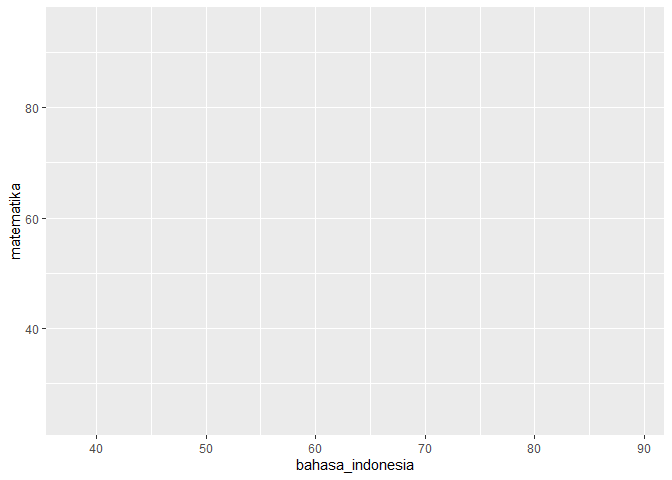
\includegraphics{modul8_files/figure-latex/unnamed-chunk-11-1.pdf}

Pendefinisian sumbu x dan y telah menghasilkan \emph{layer} baru dalam
grafik. Namun, kita masih perlu mendefinisikan bentuk dari grafik
tersebut melalui komponen \emph{geometric objects} (\texttt{geom\_*()})
sebelum grafik tersebut dapat dibaca. Tambahkan obyek geometri berupa
titik di atas \emph{layers} yang telah dibuat sebelumnya!

\begin{Shaded}
\begin{Highlighting}[]
\KeywordTok{ggplot}\NormalTok{(un_smp, }\KeywordTok{aes}\NormalTok{(}\DataTypeTok{x =}\NormalTok{ bahasa_indonesia, }\DataTypeTok{y =}\NormalTok{ matematika)) }\OperatorTok{+}
\KeywordTok{geom_point}\NormalTok{()}
\end{Highlighting}
\end{Shaded}

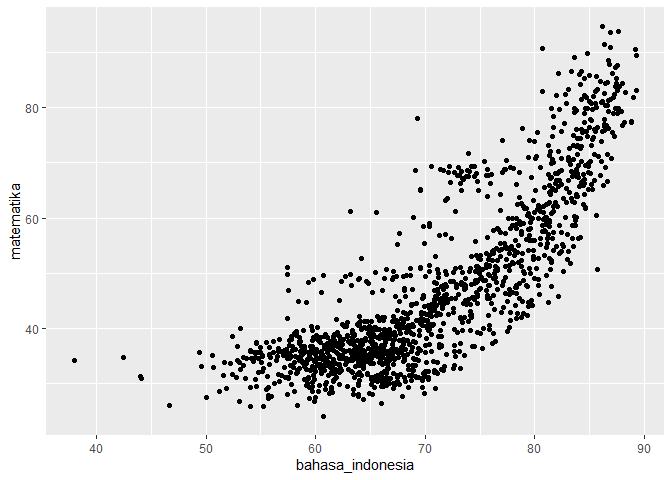
\includegraphics{modul8_files/figure-latex/unnamed-chunk-12-1.pdf}

Selamat sekarang grafik tersebut mulai dapat terbaca! Sekarang kita
ingin mengetahui bagaimanakah representasi dari status sekolah (Negeri
vs Swasta) pada grafik. Kita dapat menambahkan fungsi \texttt{aes()}
pada obyek geometri untuk melaukan hal tersebut. Dalam contoh ini kita
akan menggunakan \emph{aesthetic} berupa warna titik untuk membedakan
antar status sekolah.

\begin{Shaded}
\begin{Highlighting}[]
\KeywordTok{ggplot}\NormalTok{(un_smp, }\KeywordTok{aes}\NormalTok{(}\DataTypeTok{x =}\NormalTok{ bahasa_indonesia, }\DataTypeTok{y =}\NormalTok{ matematika)) }\OperatorTok{+}
\KeywordTok{geom_point}\NormalTok{(}\KeywordTok{aes}\NormalTok{(}\DataTypeTok{colour =}\NormalTok{ status))}
\end{Highlighting}
\end{Shaded}

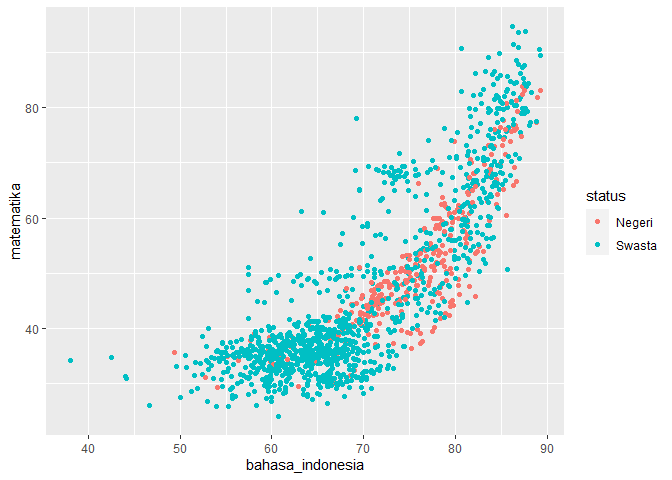
\includegraphics{modul8_files/figure-latex/unnamed-chunk-13-1.pdf}

Mudah sekali bukan? Bagaimana jika Anda ingin menambahkan informasi
jumlah peserta ujian yang direpresentasikan oleh ukuran titik dalam
grafik tersebut?

\begin{Shaded}
\begin{Highlighting}[]
\KeywordTok{ggplot}\NormalTok{(un_smp, }\KeywordTok{aes}\NormalTok{(}\DataTypeTok{x =}\NormalTok{ bahasa_indonesia, }\DataTypeTok{y =}\NormalTok{ matematika)) }\OperatorTok{+}
\KeywordTok{geom_point}\NormalTok{(}\KeywordTok{aes}\NormalTok{(}\DataTypeTok{colour =}\NormalTok{ status, }\DataTypeTok{size =}\NormalTok{ jumlah_peserta))}
\end{Highlighting}
\end{Shaded}

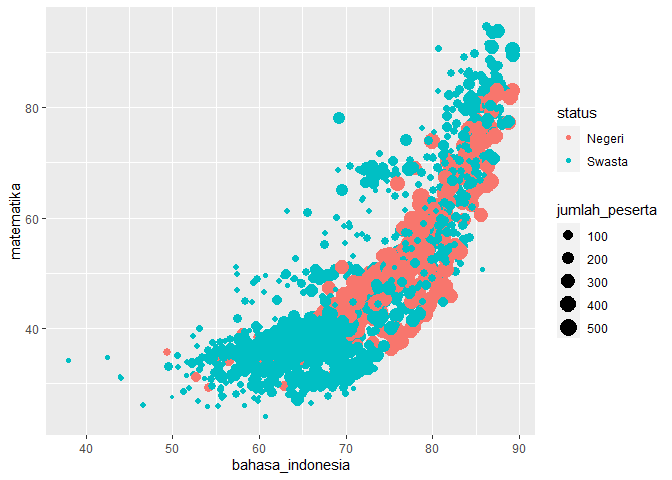
\includegraphics{modul8_files/figure-latex/unnamed-chunk-14-1.pdf}

Nampaknya jumlah peserta ujian juga memiliki hubungan dengan nilai
ujian, benarkah? Namun sayang sekali grafik tersebut sekarang telihat
sangat ``penuh'' sehingga sulit membedakan antar titik. Apakah
transparasi titik-titik tersebut dapat dimodifikasi? Ya! Anda dapat
menambahkan argumen ``alpha'' (nilai 0 hingga 1) pada obyek geometri
yang diinginkan. (Pertanyaan: Apa yang terjadi jika Anda menambahkan
argumen ``alpha'' dalam fungsi \texttt{aes()} pada obyek geometri?)

\begin{Shaded}
\begin{Highlighting}[]
\KeywordTok{ggplot}\NormalTok{ (un_smp, }\KeywordTok{aes}\NormalTok{(}\DataTypeTok{x =}\NormalTok{ bahasa_indonesia, }\DataTypeTok{y =}\NormalTok{ matematika)) }\OperatorTok{+}
\KeywordTok{geom_point}\NormalTok{(}\KeywordTok{aes}\NormalTok{(}\DataTypeTok{colour =}\NormalTok{ status, }\DataTypeTok{size =}\NormalTok{ jumlah_peserta), }\DataTypeTok{alpha =} \FloatTok{0.2}\NormalTok{)}
\end{Highlighting}
\end{Shaded}

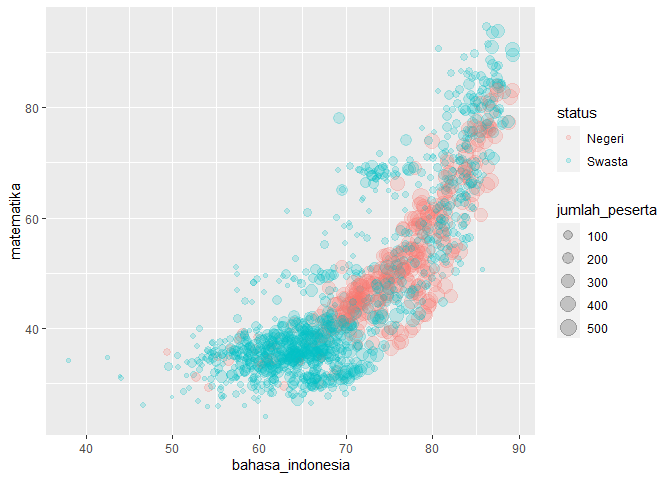
\includegraphics{modul8_files/figure-latex/unnamed-chunk-15-1.pdf}

Selanjutnya, kita ingin menganalisa lebih lanjut bagaimanakah hubungan
antar nilai ujian nasional tersebut jika dibagi per kelompok tahun.
Karena Anda sudah menggunakan empat dimensi untuk mempresentasikan data
(sumbu x, sumbu y, warna titik, ukuran titik), sekarang mungkin saatnya
Anda menggunakan pendekatan berbeda yaitu menggunakan \emph{facet}!
Tambahkanlah baris kode
\texttt{facet\_wrap(\textasciitilde{}tahun,\ scales\ =\ "free")} pada
\emph{chunk} berikut!

\begin{Shaded}
\begin{Highlighting}[]
\KeywordTok{ggplot}\NormalTok{ (un_smp, }\KeywordTok{aes}\NormalTok{(}\DataTypeTok{x =}\NormalTok{ bahasa_indonesia, }\DataTypeTok{y =}\NormalTok{ matematika)) }\OperatorTok{+}
\KeywordTok{geom_point}\NormalTok{ (}\KeywordTok{aes}\NormalTok{(}\DataTypeTok{colour =}\NormalTok{ status, }\DataTypeTok{size =}\NormalTok{ jumlah_peserta), }\DataTypeTok{alpha =} \FloatTok{0.2}\NormalTok{) }\OperatorTok{+}
\KeywordTok{facet_wrap}\NormalTok{(}\OperatorTok{~}\NormalTok{tahun, }\DataTypeTok{scales =} \StringTok{"free"}\NormalTok{)}
\end{Highlighting}
\end{Shaded}

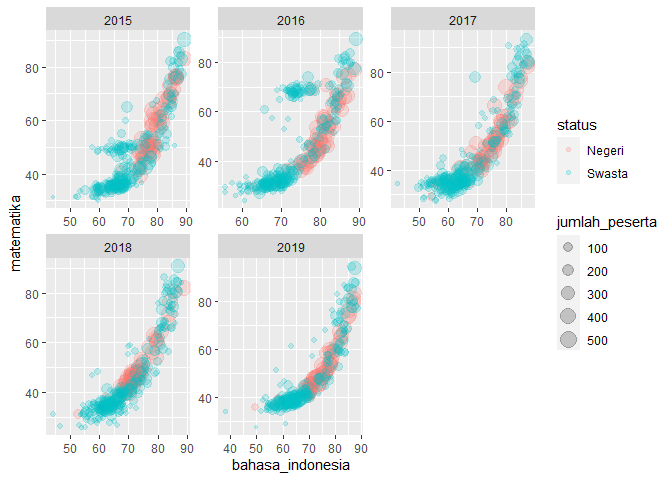
\includegraphics{modul8_files/figure-latex/unnamed-chunk-16-1.pdf}

Hasil visualisasi telah dapat memberikan analisa baru yang dapat kita
buat, Namun sayangnya Anda masih belum puas dengan grafik tersebut dalam
hal estetika. Lengkapilah \emph{chunk} berikut untuk melakukan
modifikasi estetika pada grafik tersebut! kemudian simpanlah grafik
tersebut dalam obyek R dengan nama \texttt{mtk\_vs\_ind} dan jangan lupa
cetak hasilnya pada layar.

\begin{Shaded}
\begin{Highlighting}[]
\NormalTok{mtk_vs_ind<-}\StringTok{ }\KeywordTok{ggplot}\NormalTok{(un_smp, }\KeywordTok{aes}\NormalTok{(}\DataTypeTok{x =}\NormalTok{ bahasa_indonesia, }\DataTypeTok{y =}\NormalTok{ matematika)) }\OperatorTok{+}
\KeywordTok{geom_point}\NormalTok{(}\KeywordTok{aes}\NormalTok{(}\DataTypeTok{colour =}\NormalTok{ status, }\DataTypeTok{size =}\NormalTok{ jumlah_peserta), }\DataTypeTok{alpha =} \FloatTok{0.2}\NormalTok{) }\OperatorTok{+}
\KeywordTok{facet_wrap}\NormalTok{(}\OperatorTok{~}\NormalTok{tahun, }\DataTypeTok{scales =} \StringTok{"free"}\NormalTok{) }\OperatorTok{+}
\KeywordTok{labs}\NormalTok{(}
\DataTypeTok{x =} \StringTok{"Bahasa Indonesia"}\NormalTok{,}
\DataTypeTok{y =} \StringTok{"Matematika"}\NormalTok{,}
\DataTypeTok{colour =} \StringTok{"Status sekolah"}\NormalTok{,}
\DataTypeTok{size =} \StringTok{"Jumlah Peserta"}\NormalTok{,}
\DataTypeTok{title =} \StringTok{"Matematika vs Bahasa Indonesia"}\NormalTok{,}
\DataTypeTok{subtitle =} \StringTok{"Ujian Nasional SMP di Kota Bandung 2015-2019"}\NormalTok{,}
\DataTypeTok{caption =} \StringTok{"Sumber: Open Data Kota Bandung"}
\NormalTok{) }\OperatorTok{+}
\KeywordTok{theme_light}\NormalTok{()}
\NormalTok{mtk_vs_ind}
\end{Highlighting}
\end{Shaded}

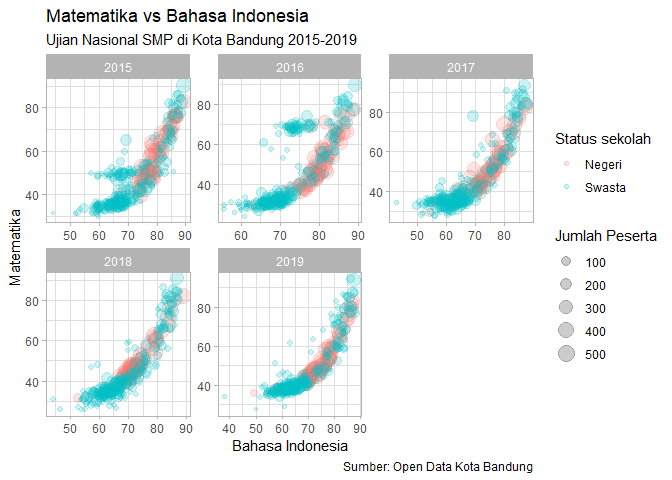
\includegraphics{modul8_files/figure-latex/unnamed-chunk-17-1.pdf}

Sekarang saatnya menyimpan grafik tersebut.

\begin{Shaded}
\begin{Highlighting}[]
\KeywordTok{ggsave}\NormalTok{(}\StringTok{"mtk_vs_indo.png"}\NormalTok{, }\DataTypeTok{plot =}\NormalTok{ mtk_vs_ind)}
\CommentTok{#> Saving 6.5 x 4.5 in image}
\end{Highlighting}
\end{Shaded}

Selamat Anda telah berhasil membuat visualisasi untuk data
\texttt{un\_smp}. Silakan Anda bereksperimen membuat grafik dengan
variabel-variabel lain atau bahkan menggunakan obyek geometri lainnya
untuk menghasilkan visulisasi data yang berbeda.

\begin{quote}
Selamat Anda telah menyelesaikan modul ini! Silakan jalankan ``Ctrl +
Shift + K'' atau klik tombol ``Knit'' untuk membuat dokumen final.
\end{quote}

\end{document}
